%%%%%%%%%%%%%%%%%%%%%%%%%%%%%%%%%%%%%%%%%
% Thin Sectioned Essay
% LaTeX Template
% Version 1.0 (3/8/13)
%
% This template has been downloaded from:
% http://www.LaTeXTemplates.com
%
% Original Author:
% Nicolas Diaz (nsdiaz@uc.cl) with extensive modifications by:
% Vel (vel@latextemplates.com)
%
% License:
% CC BY-NC-SA 3.0 (http://creativecommons.org/licenses/by-nc-sa/3.0/)
%
%%%%%%%%%%%%%%%%%%%%%%%%%%%%%%%%%%%%%%%%%

%----------------------------------------------------------------------------------------
%	PACKAGES AND OTHER DOCUMENT CONFIGURATIONS
%----------------------------------------------------------------------------------------

\documentclass[a4paper, 11pt]{article} % Font size (can be 10pt, 11pt or 12pt) and paper size (remove a4paper for US letter paper)

\usepackage[protrusion=true,expansion=true]{microtype} % Better typography
\usepackage{graphicx} % Required for including pictures\usepackage{wrapfig} % Allows in-line images
\usepackage{mathpazo} % Use the Palatino font
\usepackage[T1]{fontenc} % Required for accented characters
%\usepackage[backend=bibtex,style=verbose-trad2]{biblatex}
\usepackage{hyperref}
\usepackage{longtable}
\usepackage{array}
\usepackage{multirow}
\usepackage[utf8]{inputenc}
\usepackage{subcaption}
\usepackage[font=small]{caption}
\usepackage{units}
\usepackage{url}
\usepackage[strings]{underscore}
\usepackage[title]{appendix}
\usepackage[table, xcdraw, svgnames]{xcolor}

\linespread{1.05} % Change line spacing here, Palatino benefits from a slight increase by default

\makeatletter
\renewcommand\@biblabel[1]{\textbf{#1.}} % Change the square brackets for each bibliography item from '[1]' to '1.'
\renewcommand{\@listI}{\itemsep=0pt} % Reduce the space between items in the itemize and enumerate environments and the bibliography

\renewcommand{\maketitle}{ % Customize the title - do not edit title and author name here, see the TITLE block below
\begin{flushright} % Right align
{\LARGE\@title} % Increase the font size of the title

\vspace{50pt} % Some vertical space between the title and author name

{\large\@author} % Author name
\\\@date % Date

\vspace{40pt} % Some vertical space between the author block and abstract
\end{flushright}
}


%----------------------------------------------------------------------------------------
%	TITLE
%----------------------------------------------------------------------------------------

\title{\textbf{Specificaties}\\ % Title
Implementaties van koolstofmonoxide sensoren} % Subtitle

\author{\textsc{F. van Beusekom, M. Felida, S. van Bottenburg, J. Grobben, R. Bolding} % Author
\\{\textit{Amsterdam University of Applied Sciences\\ 
HvA\\
Sensor Netwerken: groep 5}}} % Institution

\date{20 September, 2019} % Date

%----------------------------------------------------------------------------------------
\bibliographystyle{IEEEtran}
\begin{document}
\captionsetup[figure]{labelfont={bf},name={Fig},labelsep=period}
\captionsetup{justification=centering}
\hypersetup{hidelinks=true}
\maketitle % Print the title section

%----------------------------------------------------------------------------------------
%	ABSTRACT AND KEYWORDS
%----------------------------------------------------------------------------------------

%\renewcommand{\abstractname}{Summary} % Uncomment to change the name of the abstract to something else


\vspace{10pt} % Some vertical space between the abstract and first section

%----------------------------------------------------------------------------------------
%	ESSAY BODY
%-----------------------------------------------
\newpage
\section{Inleiding}
In dit verslag worden de specificaties besproken van de te ontwikkelen sensor modules voor het project "Sensor Netwerken". Bij dit vak is het de bedoeling dat er low-power sensor modules worden ontwikkeld die de luchtkwaliteit in het HvA gebouw van de faculteit techniek meten en als netwerk informatie uitwisselen met elkaar. Binnen groep 5 is er voor gekozen om koolstofmonoxide te meten (hierna naar gerefereerd als CO). In eerste instantie was er gekozen om stikstofdioxide te meten, de onderbouwing voor de keuze om over te stappen staat beschreven in appendix A. Uiteindelijk moet iedereen van deze groep zijn eigen sensor module ontwikkelen. Aangezien het HvA gebouw van de faculteit techniek te vergelijken is met de meeste professionele werkomgevingen, wordt er voor dit onderzoek gekeken naar de gebruikelijke CO concentraties in gebouwen en hun uitschieters. Op basis daarvan worden de specificaties opgesteld voor de sensor modules.

\section{Koolstofmonoxide}
Koolstofmonoxide (CO) is een verbinding tussen koolstof en zuurstof. Het is een kleur- en geurloos gas. CO komt vrij bij een onvolledige verbranding. Dit kan erg gevaarlijk zijn voor de gezondheid omdat het gas je ongemerkt vergiftigt. Het word dan ook wel eens een "sluipmoordenaar" genoemd. 

\subsection{Ontstaan van CO}
Bij de verbranding van koolstofverbindingen ontstaat er normaal CO2. Als de verbranding onvolledig is, door bijvoorbeeld een tekort aan zuurstof, ontstaat er CO. Een veel voorkomende oorzaak van CO productie zijn niet goed afgestelde of niet goed onderhouden gas kachels en cv-ketels.

\subsection{Effecten op gezondheid}
CO is erg gevaarlijk voor de mens omdat het geur en kleurloos is. Bij inademing van CO word de zuurstofopname verstoord \cite{EffectenKoolmonoxide}. In plaats van zuurstof, bind de CO zich aan de rode bloedcellen. Omdat CO zich sterker hecht aan de rode bloedcellen dan zuurstof, word er minder zuurstof door het lichaam vervoerd. 
\\
De effecten van blootstelling aan CO zijn het gevolg van een zuurstoftekort in het bloed. Hoe meer CO er word opgenomen hoe minder zuurstof er kan worden opgenomen. 

\section{Algemene koolstofmonoxide concentraties}
Het RIVM heeft tussen april 2007 tot en met januari 2008 metingen gedaan in 1028 huishoudens. In 169 van de 1028 huishoudens werden werden er concentraties boven het detectie limiet van 1 \textit{parts per million} (hierna naar gerefereerd als \textit{ppm}) gevonden. In 8 huishoudens werden er waardes van tussen de 25 en 75 \textit{ppm}, dit waren de meest extreme waardes. in 10 andere huishoudens werden er waardes aangetroffen van tussen de 10 en 25 \textit{ppm} en in de rest van de huishoudens (verreweg de meesten) werden er waardes aangetroffen tussen de 1 en 9 \textit{ppm} \cite{RIVMhuurwoningen}. Over een werkdag van 8 uur wordt een tijdgewogen gemiddelde concentratie van 25 \textit{ppm} als grenswaarde aangenomen, over 15 minuten is dit 150 \textit{ppm}. De advies waarden van de Wereldgezondheidsorganisatie (Engels: World Health Organization, WHO) zijn 10 \textit{ppm} als tijdgewogen gemiddelde over 8 uurl en 25 \textit{ppm} over 1 uur \cite{BlootstellingaanCO}.
\subsection{Koolstofmonoxide concentraties in de HvA Leeuwenburg}
Om meer te weten te komen over de huidige manieren van meten van de koolstofmonoxide concentraties in het gebouw van de HvA faculteit techniek, is er contact gezocht het gebouwbeheer. Uit een klein gesprek is gebleken dat er momenteel alleen in de garage CO meters hangen, die wanneer er een bepaalde grenswaarde wordt overschreden (momenteel nog onbekend voor ons welke grenswaarde dat is) alarm slaan waarna vervolgens iedereen de garage moet verlaten.

\section{Luchtkwaliteit meten}
Zoals eerder werd besproken worden de te ontwikkelen sensor modules gebruikt om de luchtkwaliteit te meten. Hierbij wordt dus niet alleen bedoeld om een detector te maken die afgaat na het overschrijden van een bepaalde waarde, maar is het een doel om ook te kunnen meten wanneer je welke concentratie CO in de lucht hebt zitten en hoe ver deze concentratie ligt van de grenswaardes. Binnen groep 5 is afgesproken om de aanname te doen dat de minimale grenswaarde in delen van 1/5e gemeten moet kunnen worden. Aangezien onze sensor modules de hele dag door de CO concentraties in het gebouw moeten meten, gaan we uit van de grenswaarden voor een werk dag (8 uur lang). In dit geval komt de minimale grenswaarde voort uit de Wereldgezondheidsorganisatie (Engels: World Health Organization, WHO) en bedraagt deze 10 \textit{ppm} als tijdgewogen gemiddelde over de hele werkdag. Dit betekend dat wij de CO concentraties willen met een gevoeligheid van 2 \textit{ppm}. Het detectie limiet moet ook 1/5e zijn van de minimale grenswaarde. Dit bedraagt 2 \textit{ppm}. Aangezien CO een gas is, zullen te ontwikkelen sensor modules elektro-chemische sensoren bevatten. Elektro-chemische sensoren hebben in veel van de gevallen een response tijd, deze mag maximaal je sample tijd bedragen. Zoals hier boven staat beschreven worden de grenswaarden bepaald als een tijdgewogen gemiddelde concentratie en is het een streven om de grenswaarden op een nauwkeurigheid van 1/5e delen te kunnen meten. de minimale blootstellingsduur die wordt omschreven door het RIVM is 15 \cite{BlootstellingaanCO}. Dit betekend dat er dus elke 3 minuten een sample moet worden genomen en dus mag de response tijd van de sensor maximaal 3 minuten zijn. Bij het ontwikkelen van deze sensor modules wordt er gewerkt met het HvA-Xmega-Board. Deze heeft een spanningsregulator die een stabiele spanning van 3,3 V afgeeft \cite{xmega}, Daarom is het wenselijk als de sensor module een voedspanning heeft van zo'n 2,7 V tot 3,3 V.

\section{Specificaties}
Aan de hand van het voorgaande onderzoek zijn de volgende specificaties opgesteld. 
\begin{center}
	\begin{tabular}{ | m{5cm} | m{5cm}| } 
		\hline
		\multicolumn{2}{|c|}{Specificaties voor de implementaties van CO sensoren} \\
		\hline
		Meet bereik a: & 0 - 1000 \textit{ppm} \\
		\hline
		detectie limiet:  & <2 \textit{ppm}
		\\ 
		\hline
		detectie resolutie: & 2 \textit{ppm} 
		\\ 
		\hline
		response tijd: & < 3 minuut
		\\ 
		\hline
		Voed spanning: & min: 2,7V max: 3,3V
		\\ 
		\hline
		Maximaal vermogen: & 1 mW
		\\
		\hline
		Output gevoeligheid: & 1mV/\textit{ppm}
		\\
		\hline
	\end{tabular}
\end{center}
\newpage
\section{Ontwerpaanpak}
In dit hoofdstuk wordt aan de hand van de gekozen specificaties een ontwerpaanpak omschreven. Voordat er implementatiekeuzes kunnen worden gemaakt zal aan de hand van een gestructureerde ontwerpaanpak de functionele blokken in kaart worden gebracht. 
\subsection{Sensornode}
Voor de verschillende sensornodes geldt het volgende algemene blokdiagram (zie Figuur~\ref{fig:sensorblok}). Dit blokdiagram is vanuit de opdracht opgesteld met het doel onze beoogde grootheid te meten.  

\begin{figure}[!h]
	\centering
	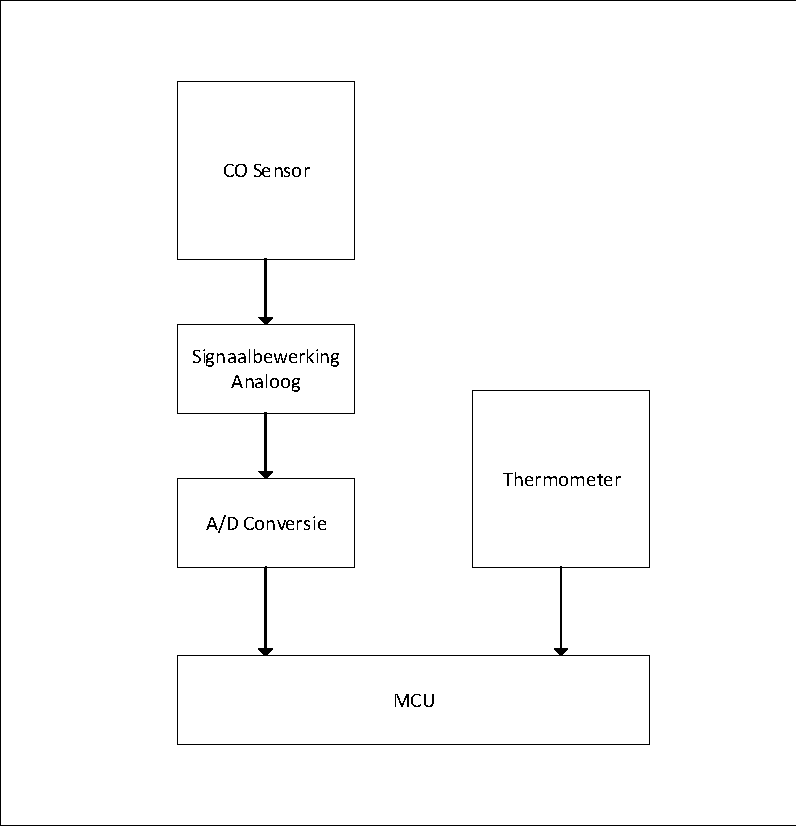
\includegraphics[width=.7\linewidth]{media/SensorTopView}
	\caption{Top-view blokdiagram van een sensor node. Deze figuur geldt voor alle vijf de CO detectie nodes.}
	\label{fig:sensorblok}
\end{figure}


\newpage
\begin{appendices}
\include{App1/NOxOnderzoek}

\section{Proof of Concept ('Work in Progress')}
Dit document beschrijft de software implementaties van groep 5 voor het vak "Sensornetwerk Ontwerp" aan de Hogeschool van Amsterdam.

Het doel van de opdracht is om een dynamisch netwerk van sensornodes te maken, waarbij in dit document de nadruk ligt op de algemene netwerkstructuur en de implementatie in MCU van de sensornodes. Hiervoor geldt over het algemeen dat het stuk software wat in dit document beschreven wordt gelijk is voor alle sensornodes. Tijdens de ontwikkeling van de individuele sensorimplementaties (vak "Sensormodule Ontwerp") kan de code afhankelijk per node worden aangepast. 

Het doel van dit document is om een 'proof of concept' te geven van de algemene netwerkstuctuur waar de sensornodes tijdens het vak "Sensormodule Ontwerp" gebruik van zullen maken.


\subsection{ISO groep}
Om te zorgen dat de nodes van de verschillende groepen elkaars datapaketten kunnen interpreteren en doorsturen zijn er afspraken gemaakt tussen de 5 groepen. Elke groep leverde 1 afgevaardigde, de 5 afgevaardigden vormden de ISO groep. De afspraken die de ISO-groep gemaakt heeft zijn opgesteld in\cite{ISO}. 

Naast afspraken over de algemene NRF-instellingen zijn er ook afspraken gemaakt over de berichttypes en de bijbehorende headers.

Bericht headers staan in de onderstaande tabel.
\subsubsection*{Message Types}
\begin{table}[h]
\begin{tabular}{|l|l|l|}
\hline
\rowcolor[HTML]{EFEFEF} 
Mask & Description           & Pipe \\ \hline
0x1  & ID Broadcast          & 0    \\ \hline
0x2  & Routine Routing Table & 1    \\ \hline
0x3  & Receive Port Data     & 1    \\ \hline
0x4  & Broadcast Reply       & 1    \\ \hline
\end{tabular}
\end{table}

\subsection{Algemene Node Programma}
Zoals besproken in de inleiding van dit document het grootste deel van de programma code voor de node MCU's gelijk. In dit hoofdstuk wordt deze code besproken. 
\subsubsection{Flowchart}
Om de algemene node-code inzichtelijk te maken is gebruik gemaakt van ene flowchart. In Figuur~\ref{fig:flowchart} is deze flowchart te zien.
\begin{figure}[!h]
	\centering	
	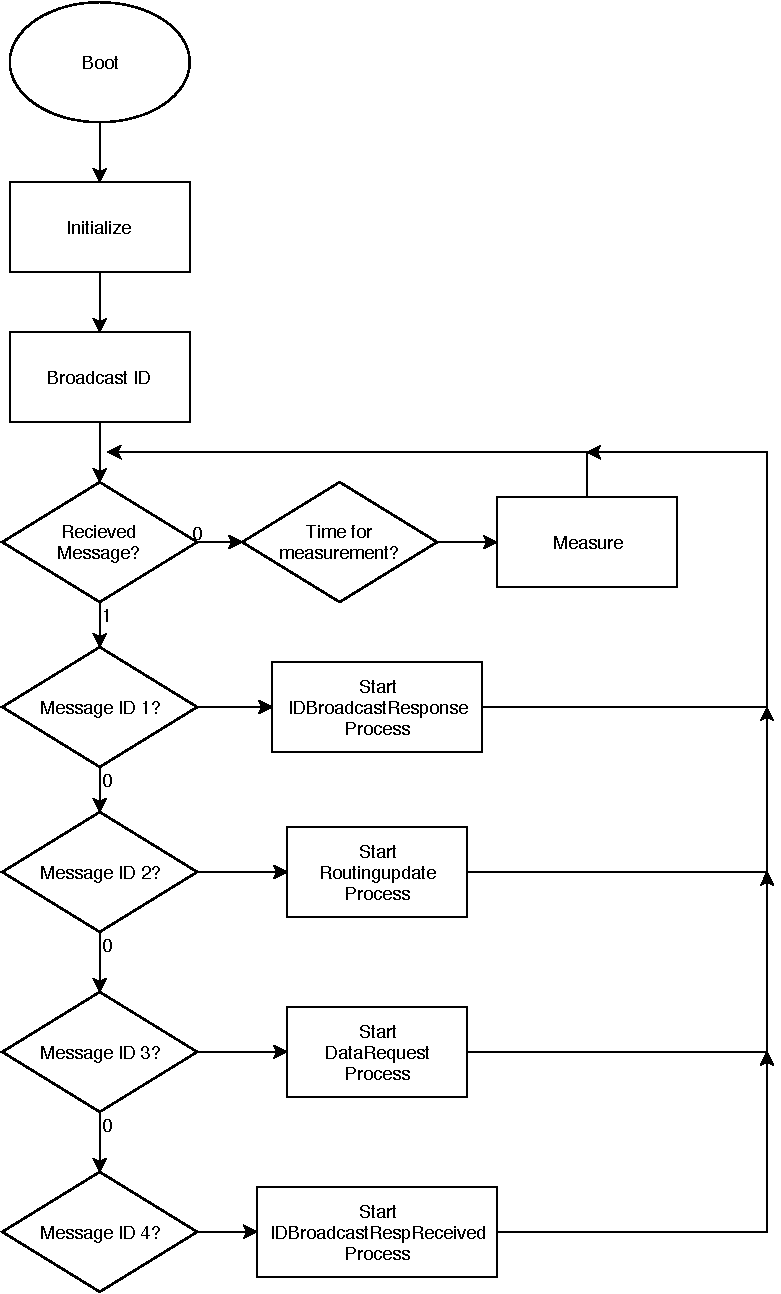
\includegraphics[width=.5\textwidth, keepaspectratio]{App2/media/Pflow.pdf}
    \caption{Nadat de node opgestart wordt (Boot) de MCU geïnitialiseerd in het blok [Initialize]
     \textbf{Figuur dient in deze versie als voorbeeld en zal geupdate worden wanneer het basis ontwerp af is.}}
    \label{fig:flowchart}
\end{figure}

\subsubsection{Statemachine}
Omdat MCU veel aan het wachten is op berichten om deze vervolgens te verwerken is gekozen als implementatie een statemachine te gebruiken. Deze is afgebeeld in Figuur~\ref{fig:Statemachine} 
Statemachine die de verschillende states laat zien waar de Xmega in komt vanaf het opstarten.
\begin{figure}[!h]
	\includegraphics[width=.8\textwidth, keepaspectratio]{App2/media/Pstate.pdf}
    \caption{ \textbf{Figuur dient in deze versie als voorbeeld en zal geupdate worden wanneer het basis ontwerp af is.}}
    \label{fig:Statemachine}
\end{figure}
\end{appendices}
\bibliography{Bronnen}
\end{document}